%\documentclass{beamer}
\documentclass[aspectratio=169]{beamer}
 
\usepackage[utf8]{inputenc}
\usetheme{Madrid}

\usepackage{biblatex}

\usepackage{mathrsfs}

\usepackage[symbols,nogroupskip,nonumberlist,sort=use]{glossaries-extra}
\usepackage{amsmath}
\usepackage{amsfonts}
\usepackage{amssymb}
\usepackage{siunitx}
\usepackage{transparent}
\usepackage{longtable,booktabs}

\usepackage{chronology}
\usepackage{epigraph}

\usepackage{caption} 
\captionsetup[table]{skip=5pt}

\sisetup{math-micro=\text{µ},text-micro=µ}
\glsxtrnewsymbol[description={Signal Segment Size}]{w}{\ensuremath{w}}
\glsxtrnewsymbol[description={Length in sample points of the Segment}]{N}{\ensuremath{N}}
\glsxtrnewsymbol[description={Number of available channels}]{C}{\ensuremath{C}}
\glsxtrnewsymbol[description={Signal Span}]{lambda}{\ensuremath{\lambda}}
\glsxtrnewsymbol[description={Sampling Frequency}]{Fs}{\ensuremath{F_s}}
\glsxtrnewsymbol[description={Length in pixel of the unit-scale patch}]{Deltas}{\ensuremath{\Delta_s}}
\glsxtrnewsymbol[description={Peak-to-peak Amplitude}]{DeltamuV}{\ensuremath{\Delta \mu V}}
\glsxtrnewsymbol[description={Signal Amplitude Scale Factor}]{gamma}{\ensuremath{\gamma}}
\glsxtrnewsymbol[description={Time Scale Factor}]{gammat}{\ensuremath{\gamma_t}}
\glsxtrnewsymbol[description={Image Height}]{Hy}{\ensuremath{H_y}}
\glsxtrnewsymbol[description={Image Width}]{Wx}{\ensuremath{W_x}}
\glsxtrnewsymbol[description={Horizontal Patch Scale}]{St}{\ensuremath{S_t}}
\glsxtrnewsymbol[description={Vertical Patch Scale}]{Sv}{\ensuremath{S_v}}
\glsxtrnewsymbol[description={Patch Height}]{Sy}{\ensuremath{\mathbf{S}_y}}
\glsxtrnewsymbol[description={Patch Width}]{Sx}{\ensuremath{\mathbf{S}_x}}
\glsxtrnewsymbol[description={Keypoint}]{kp}{\ensuremath{\mathbf{kp}}}
\glsxtrnewsymbol[description={Pixel}]{P}{\ensuremath{\mathbf{p}}}
\glsxtrnewsymbol[description={Descriptor}]{d}{\ensuremath{\mathbf{d}}}
\glsxtrnewsymbol[description={Keypoint Density}]{kpd}{\ensuremath{\mathbf{kp_d}}}
\glsxtrnewsymbol[description={Intensification Sequences Repetitions}]{ka}{\ensuremath{k_a}}
\glsxtrnewsymbol[description={Best Performing Channel}]{bpc}{\ensuremath{bpc}}
\glsxtrnewsymbol[description={Number of k-Neighbors}]{k}{\ensuremath{k}}
\glsxtrnewsymbol[description={Template Dictionary}]{T}{\ensuremath{T}}

\DeclareMathOperator*{\argmin}{arg\,min}


\newcommand*{\TitleFont}{%
      \usefont{\encodingdefault}{\rmdefault}{b}{n}%
      \fontsize{9}{20}%
      \selectfont}
      
    
%\renewcommand{\figurename}{Fig.}  
\usepackage[figurename=]{caption}

\newcommand\Fontvi{\fontsize{13}{13.2}\selectfont}

\renewcommand{\contentsname}{\centering Contents}

\newsavebox{\authbox}
\sbox{\authbox}{%
\centering
\begin{minipage}{0.33\linewidth}
\centering\normalsize
Supervisor \par
Dr. Juan Miguel Santos
\end{minipage}
\begin{minipage}{0.33\linewidth}
\centering\normalsize
Candidate \par
Rodrigo Ramele
\end{minipage}
\hfill
\begin{minipage}{0.33\linewidth}
\centering\normalsize
Cosupervisor \par
Dra. Ana Julia Villar
\end{minipage}
}
 
%Information to be included in the title page:
\title[HIST of EEG for BCI] %optional
{Histogram of Gradient Orientations of EEG Signal Plots for Brain Computer Interfaces}
 
\subtitle{Dissertation Defense}
 
\author[Ramele, Rodrigo]{ % (optional, for multiple authors)
\usebox{\authbox}
}
 
\institute[ITBA] % (optional)
{
\begin{columns}
\begin{column}{0.5\textwidth}
\hfill \includegraphics[scale=.20]{images/itbalogo.png}
\end{column}
\begin{column}{0.5\textwidth}
\Fontvi
Doctorado en Ingeniería en Informática\\
Instituto Tecnológico de Buenos Aires
\end{column}
\end{columns}
}
 
\date[Nov 29, 2018] % (optional)
{Noviembre 29 2018}


 
%\logo{\includegraphics[height=1.0cm]{images/itbalogo.png}}
 
\bibliography{Bibliography}


 
\begin{document}

%{
%\usebackgroundtemplate{\transparent{0.1}\includegraphics[width=\paperwidth]{images/brainback.png}} 
%\frame{\titlepage}
%}

\begin{frame}
\titlepage
\begin{center}
%\includegraphics[scale=0.05]{images/itba.pdf}	
%\includegraphics[height=2.0cm]{images/itbalogo.png}	
\end{center}
\end{frame}


\begin{frame}
\begin{center}
\frametitle{Outline}
\tableofcontents{}
\end{center}
\end{frame}
    
    
\section{Introduction}
\begin{frame}
\frametitle{Brain Computer Interfaces}
\begin{center}
 
\begin{figure}[]
\centering
\includegraphics[height=4cm,width=7cm]{images/Cybathlon.png}
\includegraphics[height=4cm,width=7cm]{images/Jane.jpg}\\
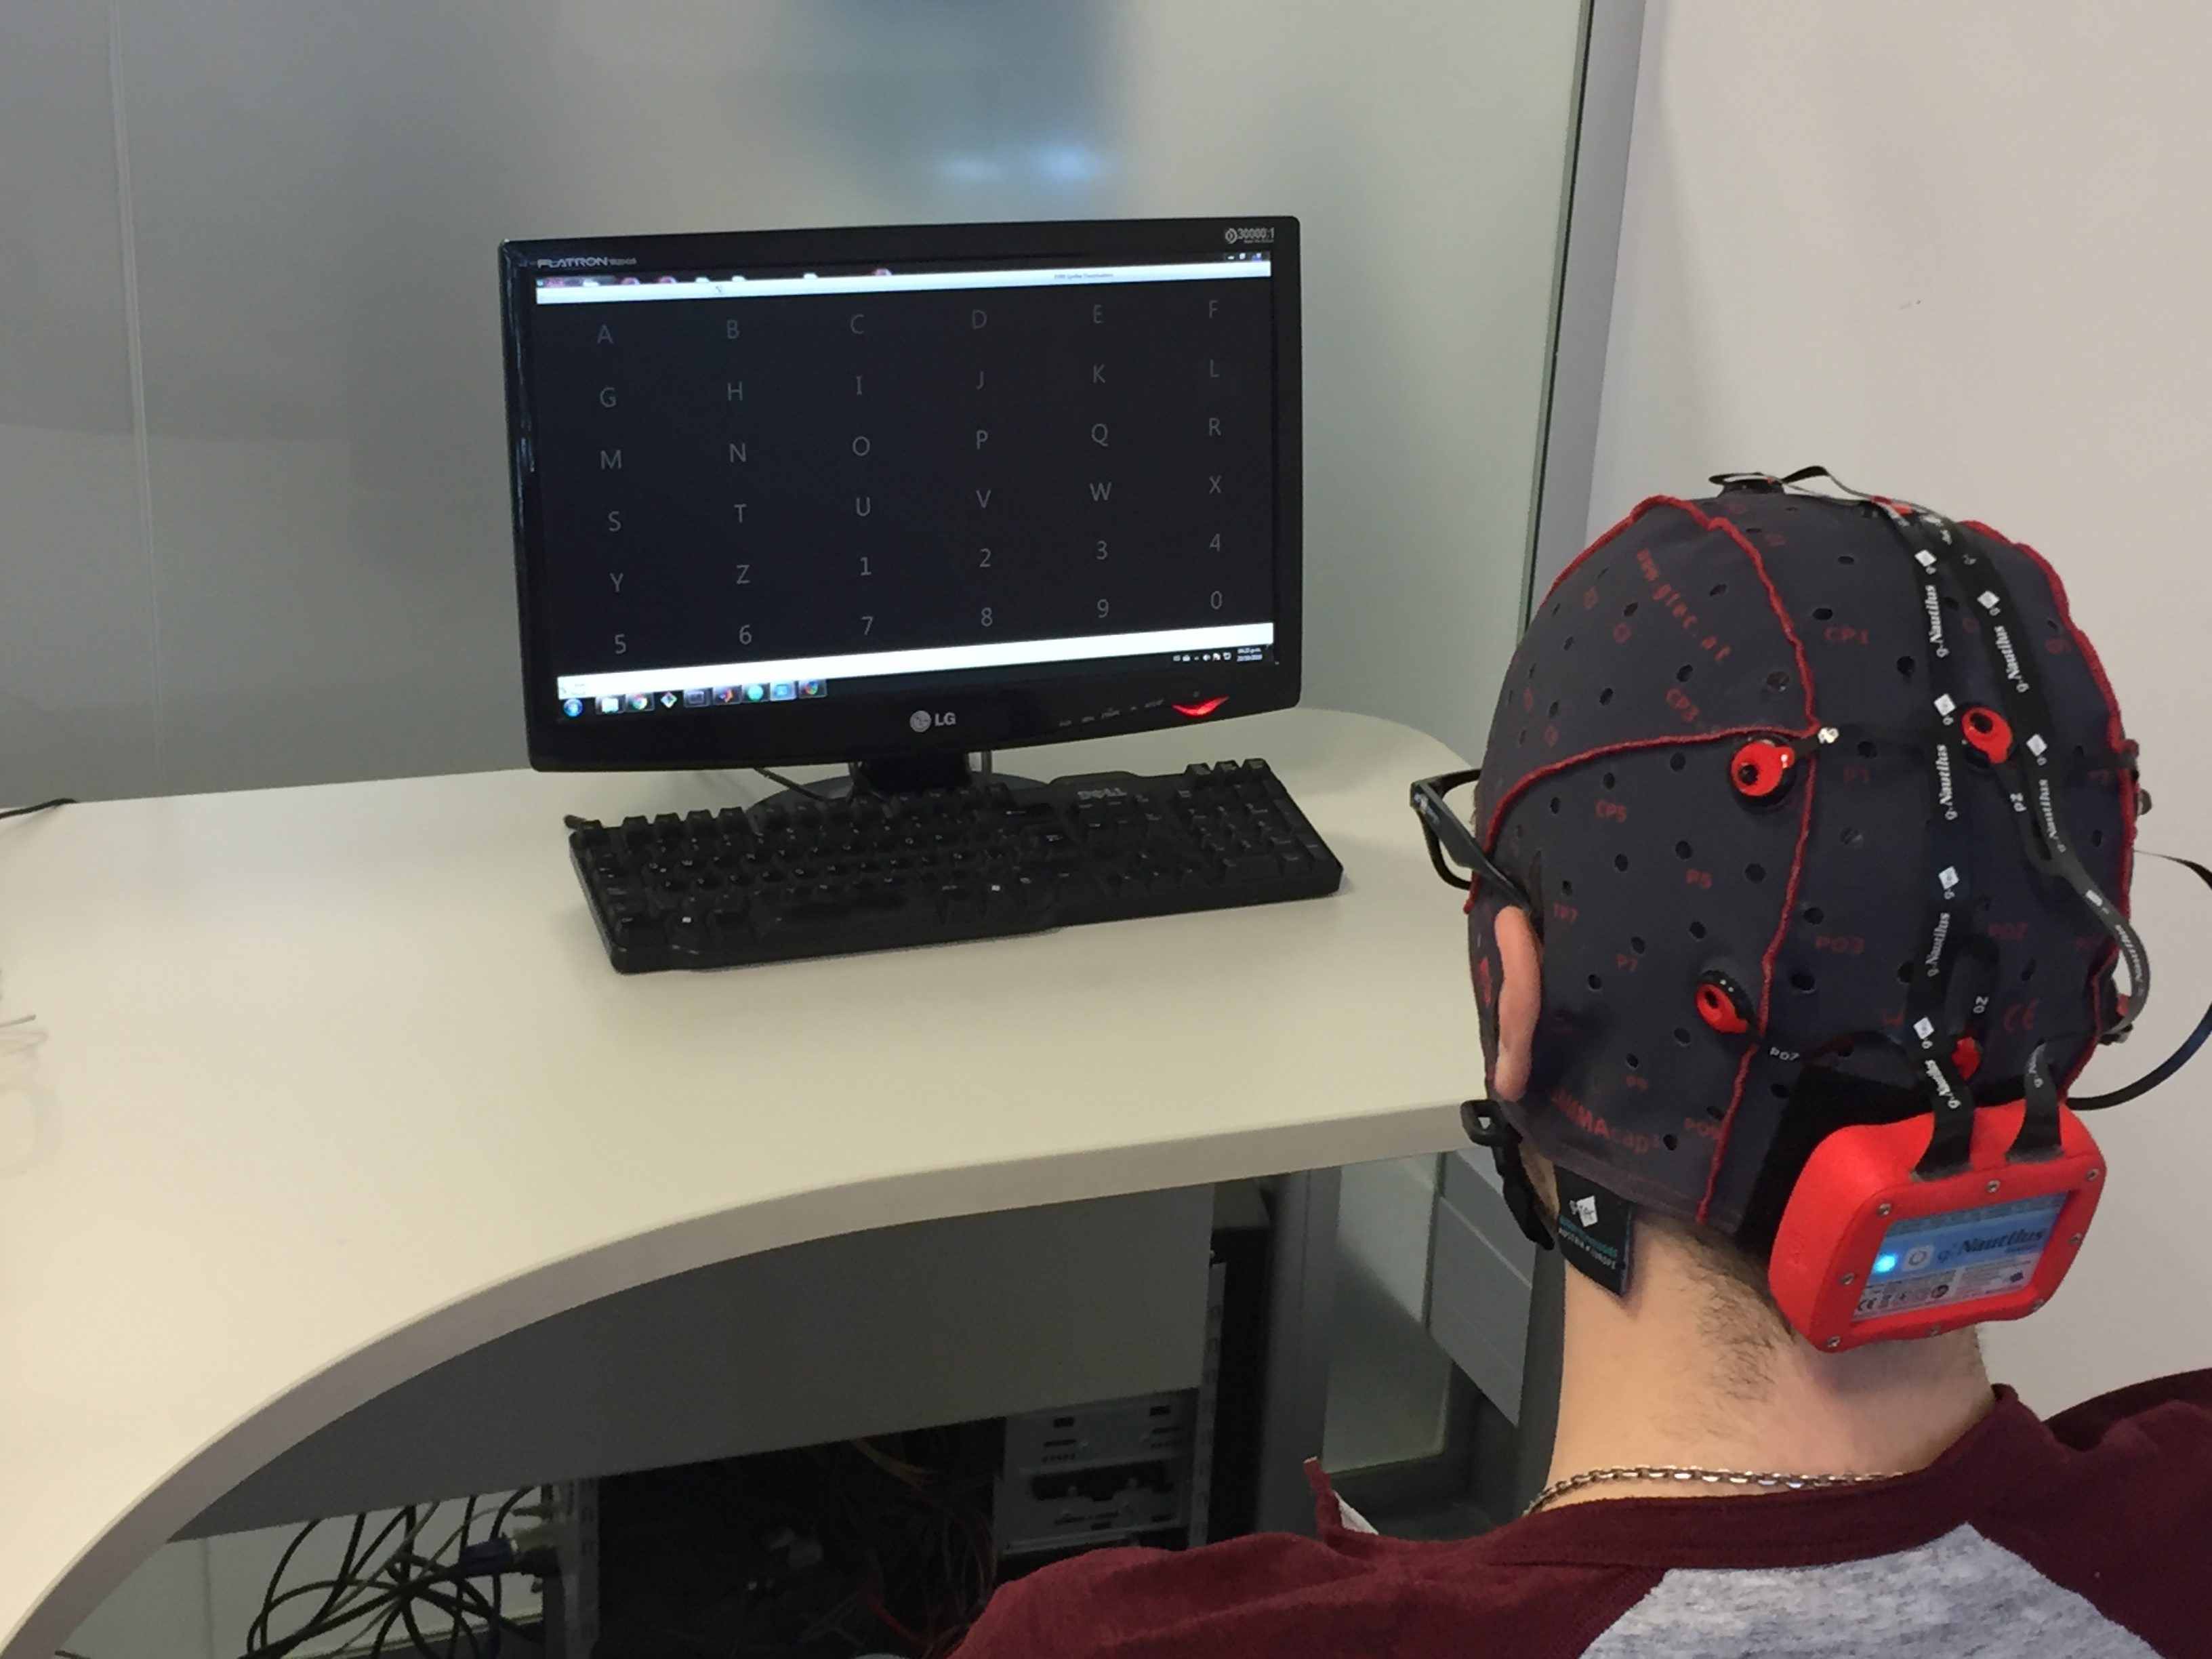
\includegraphics[height=4cm,width=7cm]{images/gTecEEGSubject.png}
\includegraphics[height=4cm,width=7cm]{images/DoC.jpg}
\caption[Wearable portable Digital Electroencephalograph]{Digital and wearable electroencephalographs.}
\label{fig:digitalelectroencephalograph}
\end{figure}

\end{center}
\end{frame}

\begin{frame}
\frametitle{Brain Computer Interfaces}
\begin{center}

\begin{chronology}[5]{1966}{2014}{90ex}[\textwidth]
\event{1966}{Kamiya, Neurofeedback for $\alpha$ waves}
\event{1969}{Fetz, Operand Conditioning}
\event{1973}{Vidal, first use of BCI word}
\event{1987}{Donchin \textbf{P300}}
\event{1989}{Hiraiwa, Bereitschaftspotentials}
\event{1991}{Wolpaw $\mu$ \textbf{Wadsworth BCI}}
\event{1993}{Pfurtscheller SMR \textbf{Graz BCI}}
\event{1995}{Jane Huggins invasive BrainGate}
\event{1997}{Anderson, Mental Tasks}
\event{1999}{Birmahuer SCP}
\event{2001}{Nicolelis, invasive BCI on primates}
\event{2003}{Middendorf, SSVEP}
\event{2006}{Millan, ErrP}
\event{2008}{Blankertz, adaptive \textbf{Berlin BCI}}
\event{2010}{Schalk, ECoG BCI}
\event{2012}{Zander, Passive BCI \textbf{pBCI}}
%\event{\decimaldate{25}{12}{2001}}{three}
\label{fig:story}
\end{chronology}

\end{center}
\end{frame}
    
\begin{frame}
\frametitle{Brain Computer Interfaces}
\begin{center}
\begin{figure}[]
\centering
\includegraphics[scale=0.4]{images/bcichart.png}
\caption[BCI Block Diagram]{General components of a BCI system.}
\label{fig:bciblockdiagram}
\end{figure}
\end{center}
\end{frame}


\begin{frame}
\frametitle{Brain Computer Interfaces}
\begin{center}
Mapa de BCI con los diferentes paradigmas y las diferentes soluciones.  También podría agregar una tabla con las velocidades alcanzadas.
\end{center}
\end{frame}

    \begin{frame}
        \frametitle{Introduction}
        \begin{center}
            \begin{itemize}
                \item BCI challenging technology.
                \item Outstanding advances but yet its push into mainstream technology has not fully materialized.
                \item More clinical and physician Involvement: devise mechanisms to help them stay in the loop.
                \item (+) speed, SNR, reliability, portability, usability.
                \item (-)  biocompatibilities, setup, training time, calibration time, subject inter/intra variability.
                \item The search for practical, relevant, and invariant features that convey good-enough information~\cite{Perdikis2014}.
                \item Ethical aspects should be revised~\cite{Yuste2017}.
            \end{itemize}
        \end{center}
    \end{frame}

\begin{frame}   
\begin{figure}[]
\centering
\includegraphics[scale=0.5]{images/BCIParadigms.png}
\caption[Wearable portable Digital Electroencephalograph]{Digital and wearable electroencephalographs.}
\label{fig:digitalelectroencephalograph}
\end{figure}
\end{frame}    
    
    \section{Motivation}
    \begin{frame}
        \frametitle{Motivation}
        \begin{center}
            \begin{itemize}
                \item This thesis tries to unravel the following question: is it possible to analyze and discriminate electroencephalographic signals by automatic processing the shape of the waveforms using the Histogram of Gradient Orientations ?
            \end{itemize}
        \end{center}
    \end{frame}
    \begin{frame}
        \frametitle{What we aim to do}
        \begin{center}
            \begin{itemize}
\begin{itemize}
\item A procedure to construct analyzable 2D-images based on one-dimensional signals.
\item An enhancement over the Histogram of Gradient Orientation technique to allow non-squared patches and to adapt it to signal plots.
\item A mapping procedure to link EEG time-series characteristics to features of 2D-images.
\item A feature extraction method for EEG signals that can be used objectively to encode a representation of the waveform.
\item A classification algorithm that use the encoded representation with the purpose of comparing and identifying waveforms for BCI applications.
\end{itemize}
            \end{itemize}
        \end{center}
    \end{frame}
    
    
\begin{frame}
\frametitle{Electroencephalography}
\begin{center}
\begin{itemize}
 \item<1-> Permutation Entropy
 \item<2-> SHCC
 \item<3-> Matching Pursuit
 \item<4-> MIDS
 \item<5-> Local Binary Patterns
 \item<6-> Peak Picking/aEEG/PAA
\end{itemize}
\end{center}
\end{frame}


\section{The Histogram of Gradient Orientations}    
\begin{frame}
\frametitle{The Histogram of Gradient Orientations}
\begin{center}
\begin{itemize}
 \item<1-> Signal Preprocessing
 \item<2-> Signal Segmentation
 \item<3-> Signal Plotting
 \item<4-> Keypoint Localization
 \item<5-> Calculation of the Histogram of Gradient Orientation
\end{itemize}
\end{center}
\end{frame}

\begin{frame}
\frametitle{The Histogram of Gradient Orientations}
\begin{center}
\begin{figure}[h!]
\centering
\includegraphics[scale=1.0]{images/imagecoordinatesystem.pdf}
\caption[Image Coordinate System]{The image coordinate system and the mapping from the signal segment.  The origin is the $(0,0)$ position at the upper-left corner of the image.  Time is represented as sample points on the horizontal axis, and the amplitude in $\mu V$ is shown on the vertical axis. Image height $H_y$ and width $W_x$ are obtained based on signal parameters.  The signal's zero-level $z(c)$ is the vertical location where the signal zero value is located. The plot of the signal is obtained by first setting the sample points on the predetermined image locations according to equation \ref{eq:images} and then applying a discrete interpolation algorithm to connect them with straight lines. The plotted waveform is a K-Complex.}
\label{fig:imagecoordinatesystem}
\end{figure}
\end{center}
\end{frame}


\begin{frame}
\frametitle{The Histogram of Gradient Orientations}
\begin{center}
\begin{figure}[h!]
\centering
\setlength\fboxsep{0pt}
\setlength\fboxrule{0.5pt}
\fbox{\includegraphics[height=2cm,width=7cm]{images/samplepoints.eps}}
\fbox{\includegraphics[height=2cm,width=7cm]{images/bresenham.eps}}\\
\fbox{\includegraphics[height=2cm,width=7cm]{images/upscaled.eps}}
\fbox{\includegraphics[height=2cm,width=7cm]{images/upsample.eps}}
\caption[Signal Plotting: Interpolation]{Generated images based on different interpolation schemes.}
\label{fig:interpolation}
\end{figure}
\end{center}
\end{frame}



\begin{frame}
\frametitle{The Histogram of Gradient Orientations}
\begin{center}
\begin{figure}[htb]
\centering
\includegraphics[height=5cm,width=5cm]{images/plotvsimage.eps}
\includegraphics[height=5cm,width=10cm]{images/sampleplot.eps}
\label{fig:plotvsimage}
\end{figure}
\end{center}
\end{frame}

\begin{frame}
\frametitle{The Histogram of Gradient Orientations}
\begin{center}
\begin{figure}[h!]
\centering
\includegraphics[width=7cm, height=6cm]{images/signalpatchkeypoint.png}
\includegraphics[width=7cm, height=6.1cm]{images/gradientsdescriptors.png}
\includegraphics[width=7cm, height=6cm]{images/samplegradients.png}
\includegraphics[width=7cm, height=6cm]{images/histogramchart.eps}
\caption[Histogram of Gradient Orientations]{Patch and vector field of oriented gradients.}.
\label{fig:sampledescriptor}
\end{figure}
\end{center}
\end{frame}

\begin{frame}
\frametitle{The Histogram of Gradient Orientations}
\begin{center}
Hence, for each spatial bin $ i,j = \{0,1,2,3\} $, corresponding to the indexes of each block $B_{i,j}$,  the orientations are accumulated in a  $3$-dimensional histogram $h$ through the following equation: 
 

\begin{equation}
 h(\theta,i,j) = \sum_{\mathbf{p}} \omega_\mathrm{ang}(\angle J(\mathbf{p}) - \theta)\, \omega_{ij}\left(\mathbf{p} - \mathbf{kp} \right)\, \left\lVert J(\mathbf{p})\right\rVert 
\label{eq:histogram}
\end{equation}

\noindent  where $\mathbf{p}$ is a pixel from within the patch,  $\theta$ is the angle bin with $ \theta \in \{0, 45, 90, 135, 180, 225, 270, 315\} $,  $ \left\lVert J(\mathbf{p}) \right\rVert $ is the norm of the gradient vector in the pixel $\mathbf{p}$, computed using finite differences, and $\angle J(\mathbf{p}) $ is the angle of the gradient vector.  The scalar $ \omega_\mathrm{ang}(\cdot) $  and vector $ \omega_{ij}(\cdot) $ functions are linear interpolations used by~\cite{Lowe2004} and \cite{Vedaldi2010} to provide a weighting contribution to eight adjacent bins. 
\end{center}
\end{frame}

\begin{frame}
\frametitle{The Histogram of Gradient Orientations}
\begin{center}
\begin{figure}[h!]
\centering
\includegraphics[width=16cm]{images/gradientorientations.pdf}
\caption[Gradient Orientations Numbering]{A scheme of the orientation's histogram computation. The first eight orientations of the first block $ B_{1,1} $, are labeled from $1$ to $8$ clockwise. The orientation of the second block $ B_{1,2} $ is labeled from $9$ to $16$.  This labeling continues left-to-right, up-down until the eight orientations for all the sixteen blocks are assigned. They form the corresponding descriptor of $128$ coordinates.  The length of each arrow represent the value of the histogram on each direction for each block.}
\label{fig:orientationsfull}
\end{figure}
\end{center}
\end{frame}


\begin{frame}
\frametitle{The Histogram of Gradient Orientations}
\begin{center}
\begin{figure}[h!]
\centering
\includegraphics[width=10cm]{images/patchgeometry.pdf}
\caption[Patch Geometry]{The scale of local patch is selected in order to capture the whole waveform, which can be scaled in the time $\gls{gammat}$ and amplitude $\gls{gamma}$ direction.  This determines appropriate horizontal $\gls{St}$ and vertical $\gls{Sv}$ patch scales.  The size of the patch is $\gls{Sx} \times \gls{Sy}$ pixels. The vertical size consists of $4$ blocks of size $\gls{Sy}$ pixels which should be high enough as to contain the signal $\gls{DeltamuV}$, the peak-to-peak amplitude of the signal component. The horizontal size includes $4$ blocks, up to $\gls{Sx}$ pixels, and should cover the entire duration in seconds of the signal waveform, $\gls{lambda}$.   }
\label{fig:patchgeometry}
\end{figure}
\end{center}
\end{frame}

   

\section{Experimental Validation}
\begin{frame}
\frametitle{BCI Paradigms}
\begin{center}
\begin{itemize}
 \item<1-> Alpha Waves Wiggles
 \item<2-> Mu Greek Letter
 \item<3-> The P300 Wave
\end{itemize}
\end{center}
\end{frame}     

\subsection{Alpha Waves wiggles}
\begin{frame}
\frametitle{Alpha Waves wiggles}
\begin{figure}[h!]
\centering
%\subfigure[Ten-fold cross-validated accuracy values, averaged across $10$ subjects.  Descriptors used for calibration are intermixed to create one template dictionary which is used for all subjects.]
\includegraphics[width=7.5cm, height=5cm]{images/Dataset1AccuracyPerChannel}
%\subfigure[Amplified image containing a sample patch located on one of the images generated for one 1-second long segment of this dataset. The keypoint location is on a sample point along the EEG trace.]
\includegraphics[width=7.5cm, height=5cm]{images/AlphaWaveSampleEEG.png}
\caption[Dataset I Classification Rate]{Dataset I: The classification accuracy is maximum on occipital channels O1 and O2. The horizontal patch scale $\gls{St}$ and the vertical patch scale $\gls{Sv}$ are set to $1$, whereas $\gls{gamma}$ and $\gls{gammat}$ are set to $2$, which corresponds to a variation of $\gls{DeltamuV} = 10$ microvolts in the signal amplitude during $\gls{lambda}=0.08$ $\si{seconds}$.}
\label{fig:alpharesultsdataseti}
\end{figure}
\end{frame}

\begin{frame}
\frametitle{Alpha Waves wiggles}
\begin{figure}[h!]
\centering
%\subfigure[Ten-fold cross-validated accuracies values for a randomly selected subject (number 12), using runs 1 and 2.]
\includegraphics[width=7.5cm, height=5cm]{images/DatasetPhysionetAccuracyPerChannel}
%\subfigure[Ten-fold cross-validated accuracy boxplots for occipital channels O1, Oz, O2 and Iz, for the 25 subjects. Mean values are around $70\%$.]
\includegraphics[width=7.5cm, height=5cm]{images/DatasetPhysionetBoxPlots}
\caption[PhysioNet Dataset Binary Classification Accuracy]{Dataset II: Classification Accuracy for segments of 1s ($\gls{N} = 160$) of EEG, between class 1 and class 2.  In this case as the sampling frequency $\gls{Fs}$ is lower, the signal span is $\gls{lambda} = 0.06$   $\si{s}$}.
\label{fig:alpharesultsdatasetii}
\end{figure}
\end{frame}





\subsection{Mu Letter}
\begin{frame}
\frametitle{Mu a Greek letter}


\end{frame}

\subsection{The P300 Wave}
\begin{frame}
\frametitle{The P300 Wave}
\begin{figure}[h!]
\centering
\includegraphics[width=15cm]{images/openvibep300matrix.png}
\caption[P300 Speller Matrix]{Example of the $6 \times 6$ Speller Matrix from the OpenVibe software.  Rows and columns flash in random permutations.}
\label{fig:p300matrix}
\end{figure}

\end{frame}    

\begin{frame}
\frametitle{The P300 Wave}
\begin{center}
\begin{figure}[htb]
\centering
\includegraphics[width=15cm]{images/classificationgraph.pdf}
\caption[P300 Speller Matrix Letter Identification]{For each column and row, an averaged, standardized and scaled signal $\tilde{x}^l(n,c)$ is obtained from the segments $S_i^l$  corresponding to the $\gls{ka}$ intensification sequences with $ 1 \leq i \leq k_a $ and location $l$ varying between $1$ and $12$. From the averaged signal, the image $I^{(l,c)}$ of the signal plot is generated and each descriptor is computed.  By comparing each descriptor $\mathbf{q}$  against the set of templates, the P300 ERP can be detected, and finally the desired letter from the matrix can be inferred.}
\label{fig:classification}
\end{figure}
\end{center}
\end{frame}     

\begin{frame}
\frametitle{The P300 Wave}
\begin{center}
\textbf{Step D:} Match to the calibration template $T^{bpc}$ by computing  

\begin{equation}
\hat{row} = \arg \min_{l \in \{1,\dots,6\}} \sum_{h=1}^{\gls{k}}  {\left\lVert \mathbf{q}^{(l,bpc)} -  \mathbf{d}_{h}^{(bpc)} \right\rVert}  ^{2}
\label{eq:multiclassificationrow}
\end{equation}

\noindent and

\begin{equation}
\hat{col} = \arg \min_{l \in \{7,\dots,12\}} \sum_{h=1}^{\gls{k}}  {\left\lVert \mathbf{q}^{(l,bpc)} -  \mathbf{d}_{h}^{(bpc)} \right\rVert}  ^{2}
\label{eq:multiclassificationcol}
\end{equation}

\noindent with $\mathbf{d}_{h}^{(bpc)}$ belonging to the set $N_T( \mathbf{q}^{(l,bpc)}  )$, which is defined, for the best performing channel,  as $N_T(\mathbf{q}^{(l,bpc)} ) = \{ \mathbf{d}_{h}^{(bpc)} \in T^{bpc} /  \mathbf{d}^{(bpc)} $  is the $\gls{k}$-nearest neighbor of $ \mathbf{q}^{(l,bpc)} \}$.  This procedure is a unary classification scheme, an adapted version of the algorithm described in Section~\ref{nbnn} to the letter identification required in the BCI-Based P300 Speller implementation.
\end{center}
\end{frame}   


\begin{frame}
\frametitle{The P300 Wave}
\begin{center}
\begin{itemize}
 \item<1-> Dataset I - P300 ALS Public Dataset
 \item<2-> Dataset II - P300 for healthy subjects
 \item<3-> Dataset III - P300 Pseudo-Real Dataset Generation
 \item<4-> Dataset IV - P300 Dataset IIb BCI Competition II (2003)
\end{itemize}
\end{center}
\end{frame} 


\begin{frame}
\frametitle{The P300 Wave}
\begin{center}
\begin{table}[h!]
\caption[Dataset I - Single Channel Character Recognition Rates]{Dataset I: Character recognition rates for the public dataset of ALS patients using HIST calculated from single-channel plots.  Performance rates using single-channel signals with the SVM classifier are shown for comparison.  The best performing channel $bpc$ for each method is visualized}
\centering
%% \tablesize{} %% You can specify the fontsize here, e.g.  \tablesize{\footnotesize}. If commented out \small will be used.
\begin{tabular}{c|cc|cc}
\toprule
\textbf{Participant}	&  $bpc$ 	&  HIST &  $bpc$	&  Single Channel SVM \\
\midrule
1     &     Cz   &   $35\%$    &  Cz   & $15\%$   \\
2     &     Fz   &   $85\%$      &  PO8   & $25\%$   \\
3     &     Cz   &   $25\%$    &  Fz   & $5\%$   \\
4     &     PO8 &   $55\%$   &  Oz   & $5\%$    \\
5     &     PO7 &   $40\%$    &  P3   & $25\%$   \\
6     &     PO7 &   $60\%$  &  PO8   & $20\%$    \\
7     &     PO8 &   $80\%$   &  Fz   & $30\%$     \\
8     &     PO7 &   $95\%$     &  PO7   & $85\%$ \\

%\bottomrule
\end{tabular}
\label{tab:resultsals}
\end{table}
\end{center}
\end{frame} 


\begin{frame}
\frametitle{The P300 Wave}
\begin{center}
\begin{figure}[h!]
\centering
\includegraphics[width=10cm]{images/performance.eps}
\caption[Dataset I ALS Patients Dataset P300 Performance Curves]{Performance curves for the eight subjects included in the dataset I of ALS patients.  Three out of eight subjects achieved the necessary performance to implement a valid P300 speller.}
\label{fig:performance}
\end{figure}
\end{center}
\end{frame} 


\begin{frame}
\frametitle{The P300 Wave}
\begin{center}
\begin{table}[h!]
\caption[Dataset II - Single Channel Character Recognition Rates]{Dataset II: Character recognition rates and $bpc$  using HIST calculated from  single-channel signals.  Performance rates using single-channel signals with the SVM classifier are shown for comparison.}
\centering
%% \tablesize{} %% You can specify the fontsize here, e.g.  \tablesize{\footnotesize}. If commented out \small will be used.
\begin{tabular}{c|cc|cc}
\toprule
\textbf{Participant}	&  $bpc$	&  HIST &  $bpc$	&  Single Channel SVM \\
\midrule
1     &     Oz   &   $40\%$  &  Cz   &  $10\%$    \\
2     &     PO7   &   $30\%$      &  Cz   & $5\%$   \\
3     &     P4   &   $40\%$    &  P3   & $10\%$    \\
4     &     P4 &   $45\%$    &  P4   & $35\%$     \\
5     &     P4 &   $60\%$  &  P3   & $10\%$     \\
6     &     Pz &   $50\%$ &  P4   & $25\%$     \\
7     &     PO7 &   $70\%$  &  P3   & $30\%$     \\
8     &     P4 &   $50\%$    &  PO7   & $10\%$    \\

%\bottomrule
\end{tabular}
\label{tab:resultsown}
\end{table}
HIST method has an improved performance at letter identification than SVM that process the signals on a channel by channel strategy (Wilcoxon signed-rank test, $p =  0.004$ for both datasets).
\end{center}
\end{frame} 


\begin{frame}
\frametitle{The P300 Wave}
\begin{center}
\begin{table}[h!]
\caption[Dataset I - Comparisons of Character Recognition Rates]{Character recognition rates and the best performing channel $bpc$ for the public dataset I  using the HIST versus performance rates obtained by SWLDA and SVM classification algorithms with a multichannel concatenated feature.}
\centering
%% \tablesize{} %% You can specify the fontsize here, e.g.  \tablesize{\footnotesize}. If commented out \small will be used.
\begin{tabular}{c|cc|c|c}
\toprule
%\textbf{Participant}	&  \textbf{BPC}	& \multicolumn{2}{c}{Character Recognition Rates}\\
%\cline{1-5} \\
\textbf{Participant}	&  $bpc$	&  HIST & Multichannel SWLDA & Multichannel SVM \\
                                    &  for HIST        &           &                                       &   \\
\midrule
1     &     Cz   &   $35\%$  & $45\%$  & $40\%$\\
2     &     Fz   &   $85\%$  & $30\%$   & $50\%$   \\
3     &     Cz   &   $25\%$  & $65\%$ & $55\%$   \\
4     &     PO8 &   $55\%$ & $40\%$  & $50\%$   \\
5     &     PO7 &   $40\%$ & $35\%$  & $45\%$   \\
6     &     PO7 &   $60\%$ &  $35\%$  & $70\%$   \\
7     &     PO8 &   $80\%$ & $60\%$   & $35\%$   \\
8     &     PO7 &   $95\%$  & $90\%$   & $95\%$  \\

%\bottomrule
\end{tabular}
\label{tab:resultsalsswlda}
\end{table}
\end{center}
\end{frame} 


\begin{frame}
\frametitle{The P300 Wave}
\begin{center}
\begin{figure}[h!]
\centering
\includegraphics[width=10cm]{images/boxplots.png}
\caption[Dataset I and II Performance Boxplots]{Boxplots obtained for the methods HIST and multichannel SVM and SWLDA for the Datsets I and II.  The achieved performance for the HIST method is similar to the performace obtained for the other methods (Quade test with $p=0.55$).}
\label{fig:boxplots}
\end{figure}
\end{center}
\end{frame} 

\begin{frame}
\frametitle{The P300 Wave}
\begin{center}
\begin{table}[h!]
\caption[Dataset II - Comparisons of Character Recognition Rates]{Character recognition rates and the best performing channel $bpc$ for the  dataset II  using HIST versus performance rates obtained by SWLDA and SVM classification algorithms with a multichannel concatenated feature.}
\centering
%% \tablesize{} %% You can specify the fontsize here, e.g.  \tablesize{\footnotesize}. If commented out \small will be used.
\begin{tabular}{c|cc|c|c}
\toprule
%\textbf{Participant}	&  \textbf{BPC}	& \multicolumn{2}{c}{Character Recognition Rates}\\
%\cline{1-5} \\
\textbf{Participant}	&  $bpc$ 	&  HIST & Multichannel SWLDA & Multichannel SVM  \\
                                    &  for HIST        &           &                                       &   \\
\midrule
1     &     Oz   &     $40\%$  &     $65\%$  &     $40\%$ \\
2     &     PO7   &     $30\%$ &   $15\%$  &     $10\%$ \\
3     &     P4   &     $40\%$ &     $50\%$  &     $25\%$ \\
4     &     P4   &     $45\%$ &     $40\%$  &     $20\%$ \\
5     &     P4   &      $60\%$ &    $30\%$  &     $20\%$ \\
6     &     Pz   &      $50\%$ &    $35\%$  &     $30\%$ \\
7     &     PO7   &      $70\%$ &  $25\%$  &     $30\%$ \\
8     &     P4   &      $50\%$ &    $35\%$  &     $20\%$ \\

%\bottomrule
\end{tabular}
\label{tab:resultsownswlda}
\end{table}
\end{center}
\end{frame} 

\begin{frame}
\frametitle{The P300 Wave}
\begin{center}
\begin{figure}[h!]
\centering
\includegraphics[width=15cm]{images/subject.png}\label{subject8}
\caption[Sample P300 Patches]{Ten sample P300 template patches for Subjects 8 (A) and 3 (B) of the public Dataset I of ALS patients.}  %Downward deflection is positive polarity. 
\label{fig:p300templates}
\end{figure}
\end{center}
\end{frame} 

\begin{frame}
\frametitle{The P300 Wave}
\begin{center}
Additionally, the stability of the P300 component waveform has been extensively studied in patients with ALS \cite{SellersandEmanuelDonchin2006,TomohiroMadarame2008,Nijboer2009,Mak2012,McCane2015} where it was found that these patients have a stable P300 component, which were also sustained across different sessions.  In line with these results we do not find evidence of a difference in terms of the performance obtained by analyzing the waveforms, by using the HIST method, for the group of patients with ALS and the healthy group of volunteers (Mann-Whitney U Test, $p=0.46$). Particularly, the best performance is obtained for a subject from the ALS dataset for which, based on visual observation, the shape of they P300 component is consistently identified.
\end{center}
\end{frame} 
    

    
    \section{Conclusion}
    \begin{frame}
        \frametitle{Dissertation Contributions}
        \begin{center}
            \begin{itemize}
                \item A procedure to construct analyzable 2D-images based on one-dimensional signals.
                \item The introduction of the HIST method as an enhancement on the SIFT technique to allow non-squared patches and to adapt it to signal plots.
                \item A mapping procedure to link EEG time-series characteristics to features of 2D-images.
                \item A feature extraction method for EEG signals that can be used objectively to encode a representation of the waveform.
                \item A classification algorithm that use the encoded representation with the purpose of comparing and identifying waveforms for BCI applications.
            \end{itemize}
        \end{center}
    \end{frame}    
    
\begin{frame}
\frametitle{Conclusion}
\begin{center}
\begin{itemize}
\item EEG Waveforms can be analyzed by this method.
\item Oscillatory processes can be studied by this methodology.
\item The stability of ERP transient components can be studied objetively with the proposed methology.
\end{itemize}
\end{center}
\end{frame}    
    
    
    \section{References}
    \begin{frame} %Biblio
        \frametitle{References}

    \end{frame}
    
    
        \section{Questions}
    \begin{frame} %Biblio
        \frametitle{Questions}
        \begin{center}
        \LARGE Questions?
        \end{center}
    \end{frame}

\begin{frame}
\frametitle{Sample frame title}
This is a text in first frame. This is a text in first frame. This is a text in first frame.
\end{frame}


\begin{frame}
\frametitle{Sample frame title}
This is a text in second frame. 
For the sake of showing an example.
 
\begin{itemize}
 \item<1-> Text visible on slide 1
 \item<2-> Text visible on slide 2
 \item<3> Text visible on slide 3
 \item<4-> Text visible on slide 4
\end{itemize}
 
\end{frame}

\begin{frame}
\frametitle{Sample frame title}
\begin{equation}
 \omega_\mathrm{ang}(\alpha) = \sum_{r=-1}^{1} \omega \bigg ( \frac{8\alpha}{2\pi} + 8r \bigg )
\label{eq:wang}
\end{equation}
\end{frame}

\begin{frame}
\frametitle{Sample frame title}
 
In this slide, some important text will be
\alert{highlighted} beause it's important.
Please, don't abuse it.
 
\begin{block}{Remark}
Sample text
\end{block}
 
\begin{alertblock}{Important theorem}
Sample text in red box
\end{alertblock}
 
\begin{examples}
Sample text in green box. "Examples" is fixed as block title.
\end{examples}
\end{frame}

    \begin{frame}
        \begin{center}
            \LARGE Method   
        \end{center}
    \end{frame}
    
    \begin{frame}
        \frametitle{Signal Transformation}
        \begin{center}           

Single Channel transformation of the EEG multichannel time series matrix into an image
\begin{equation}
\mathscr{T}\{x(t,c,V)=0\} \mapsto I(z_1,z_2, \mathcal{C}, \mathcal{I}) = 0
\end{equation}
where $ t $ is time, $ c $ is the specified channel, $ V $ is the voltage value for the signal, $ \mathcal{C} $ is the color channel for an image and  $ \mathcal{I} $ is the pixel value intensity.

\vspace{17pt}

Plot Generation: The EEG matrix is transformed to a binary bidimensional image $ (t,c,V) \mapsto (t, V, Grey, \mathcal{I}) $ with $\mathcal{I} = 0$ or  $\mathcal{I} = 255$ for each $ c $.

		\end{center}
	\end{frame}
	
	\begin{frame}
	\frametitle{Signal Transformation: Visually centering the signal over the image.}
	\begin{center}

First the non-zero media is removed from the signal.
	
\begin{equation}
\tilde{x}(t,c) = \lfloor  \delta .(  x(t,c) - \bar{x}(c)  )   \rfloor 
\end{equation}
	
And the signal is centered on the image

\begin{equation}
h(c) = ( \max{} \tilde{x}(t,c) - \min{} \tilde{x}(t,c) ) + \sigma 
\end{equation}

\begin{equation}
Z(c) = \lfloor \frac{h(c)}{2} \rfloor - \lfloor \frac{\max{} \tilde{x}(t,c) + \min{} \tilde{x}(t,c)}{2} \rfloor 
\end{equation}

where $ t $ is time, $ \delta $ is scale factor,  $ c $ is the channel parameter, $ x(t,c) $ is the EEG matrix whereas $ \bar{x}(c) $ is the mean value for each channel,  $ h(c) $ is the height of the image in pixels, $ \sigma $ is the descriptor size and $ Z(c) $ is the horizontal pixel at which the zero value of the signal will be located.

	\end{center}
	\end{frame}

	\begin{frame}
	\frametitle{Signal Transformation: Binary Image generation.}
	\begin{center}
	
\begin{equation}
I(z_1,z_2) = \left\{ \begin{array}{rl}
255      & z_1 = \delta \cdot t;  z_2 = \tilde{x}(t,c) + Z(c)   \\
0   & \mbox{otherwise}
\end{array}\right. 
\end{equation}

		\includegraphics[scale=2]{images/SignalSample.png} 
		\includegraphics[scale=2]{images/SignalSample2.png} 
		
% \eqno{(2)}

        \end{center}
    \end{frame}


%    \begin{frame}
  %      \frametitle{Signal Transformation}
 %       \begin{center}           
   %     \includegraphics[scale=4]{images/SignalTransformation.png} 
     %   \end{center}
    %\end{frame}
    
    \begin{frame}
    \frametitle{Features: SIFT\footfullcite{Lowe 2004} Descriptors}
    
    Scale Invariant Feature Transform Descriptors are local features of an image that represents gradient changes in intensities.  They are 128-dimensional vectors that contains the histograms of relative gradient directions on each of the blocks that each patch is divided (4x4=16 blocks, 8 rotational directions on each).  A single scale ($ \sigma = 1 $) is composed of 4 blocks of 3 pixels on each side (12x12).
    
        \includegraphics[scale=0.5]{images/sift-conv-vlfeat.png}     
    \end{frame}
    
    \begin{frame}
        \frametitle{SIFT Descriptors}
        \begin{center}
   			\begin{figure}[thpb]
      			\centering
      			\setlength\fboxsep{0pt}
	  			\setlength\fboxrule{0.5pt}
       			\fbox{\includegraphics[scale=0.7]{images/BaselineDescriptor.png}}
      			\caption{\centering SIFT Descriptor $ [ z_1, z_2, \theta, \sigma ] $ where $ (z_1, z_2) $ are the 2D coordinates where the \textit{Keypoint} is located, $ \theta $ is the descriptor general orientation and $ \sigma $ is the descriptor size. }
      			\label{figure1}
   			\end{figure}        
        \end{center}
    \end{frame}   
    
    \begin{frame}
        \frametitle{SIFT Descriptors}
        \begin{center}
   			\begin{figure}[thpb]
      		\centering
      		\setlength\fboxsep{0pt}
	  		\setlength\fboxrule{0.5pt}
       		\fbox{\includegraphics[scale=0.8]{images/BaselineDescriptorZoom.png}}
      		\caption{\centering  SIFT Descriptor with its corresponding gradient tendencies.}
      		\label{figure1}
   			\end{figure}        
        \end{center}
    \end{frame}   
    
    \begin{frame}
        \frametitle{SIFT Descriptors}
        \begin{center}
   			\begin{figure}[thpb]
      		\centering
      		\setlength\fboxsep{0pt}
	  		\setlength\fboxrule{0.5pt}
       		\fbox{\includegraphics[scale=0.6]{images/EasyDescriptorSample1.png}}
       		\fbox{\includegraphics[scale=0.6]{images/EasyDescriptorSample2.png}}
      		\caption{\centering Sample Descriptors from artificial signals.}
      		\label{figure1}
   			\end{figure}        
        \end{center}
    \end{frame}       
        
    \begin{frame}
        \frametitle{SIFT Descriptors}
        \begin{center}
   			\begin{figure}[thpb]
      		\centering
      		\setlength\fboxsep{0pt}
	  		\setlength\fboxrule{0.5pt}
       		\fbox{\includegraphics[scale=0.48]{images/BaselineDescriptorValues2.png}}
      		\caption{\centering Sample descriptor values of the given patch.}
      		\label{figure1}
   			\end{figure}        
        \end{center}
    \end{frame}   
    
    %\begin{frame}
     %   \frametitle{SIFT Descriptors}
       % \begin{center}
   		%	\begin{figure}[thpb]
      	%		\centering
      	%		\setlength\fboxsep{0pt}
	  	%		\setlength\fboxrule{0.5pt}
       	%		\fbox{\includegraphics[scale=0.4]{images/BaselineDescriptorRepresentation.png}}
      	%		\caption{\centering Descriptor values and their representation as intensity gradients.}
      	%		\label{figure1}
   		%	\end{figure}        
       % \end{center}
    %\end{frame}   
    
    \begin{frame}
        \frametitle{Keypoint Localization}
        \begin{center}
   			\begin{figure}[thpb]
      			\centering
      			\setlength\fboxsep{0pt}
	  			\setlength\fboxrule{0.5pt}
       			%\fbox{\includegraphics[scale=1.5]{images/KeypointLocations2.png}}
       			\fbox{\includegraphics[scale=0.58]{images/SignalWithFullDescriptors.png}}
      			\caption{\centering Keypoints are $ (z_1, z_2) $ points on the image where descriptors are extracted.}
      			\label{figure1}
   			\end{figure}        
        \end{center}
    \end{frame}      
     
     
    
    \begin{frame}
        \frametitle{Classification}
        \begin{center}
            \begin{itemize}
                \item Discriminative Semi-supervised classification method was used:  Naive Bayes Nearest Neighbor, NBNN\footfullcite{Boiman, Shechtman, Irani 2008} algorithm:
			\end{itemize}
                
                
$$
\hat{C} = \argmin_C \sum {\lVert  d_i - NN_C(d_i)  \rVert}^2 \eqno{(3)}
$$                 
   
where $ \hat{C} $ is estimated Class to which this image (and underlying EEG signal windows) should belong whereas $ d_i $ is the i-th descriptor obtained from the query image and  $ NN_C(d_i)  $ is the near neighbor descriptor for each class.         
                
        \end{center}
    \end{frame}
    
    % Graph NBNN
    \begin{frame}
        \frametitle{Classification}
        \begin{center}
            \item \includegraphics[scale=0.38]{images/NBNNMethod1.png}     
        \end{center}
    \end{frame}
    
    \begin{frame}
        \frametitle{Classification}
        \begin{center}
            \item \includegraphics[scale=0.38]{images/NBNNMethod2.png}        
        \end{center}
    \end{frame}
    
    \begin{frame}
        \frametitle{Classification}
        \begin{center}
            \item \includegraphics[scale=0.38]{images/NBNNMethod3.png}    
        \end{center}
    \end{frame}    

    \begin{frame}
        \frametitle{Classification}
        \begin{center}
            \item \includegraphics[scale=0.38]{images/NBNNMethod4.png}     
        \end{center}
    \end{frame}    
    
    \begin{frame}
        \frametitle{Classification}
        \begin{center}
            \item \includegraphics[scale=0.38]{images/NBNNMethod5.png}     
        \end{center}
    \end{frame}    
    
    
    \begin{frame}
        \begin{center}
            \LARGE Offline Results   
        \end{center}
    \end{frame}
    
    \begin{frame}
        \frametitle{Dataset I: Subject Independent $\alpha $ Waves \footfullcite{Ramele, Villar, Santos 2014}}        
   \begin{figure}[thpb]
      \centering
      \setlength\fboxsep{0pt}
	  \setlength\fboxrule{0.5pt}
       \fbox{\includegraphics[scale=0.46]{images/Dataset1AccuracyPerChannel.eps}}
      \caption{\centering 10-Fold Cross validated accuracy values for 10 subjects.}
      \label{figure2}
   \end{figure}   
    \end{frame}
    
    
    \begin{frame}
      \frametitle{Dataset II: EEG Dataset, Runs 1 and 2 \footfullcite{Goldberg et al 2000, Schalk 2004}}
   \begin{figure}[thpb]
      \centering
      \setlength\fboxsep{0pt}
	  \setlength\fboxrule{0.5pt}
       \fbox{\includegraphics[scale=0.58]{images/DatasetPhysionetAccuracyPerChannel}}
      \caption{\centering 10-Fold Cross validated accuracies values for one random subject.}
      \label{figure2}
   \end{figure}          
    \end{frame}    

    \begin{frame}
    \frametitle{Dataset II: EEG Dataset, Runs 1 and 2 \footfullcite{Goldberg et al 2000, Schalk 2004}}
   \begin{figure}[thpb]
      \centering
      \setlength\fboxsep{0pt}
	  \setlength\fboxrule{0.5pt}
       \fbox{\includegraphics[scale=0.63]{images/DatasetPhysionetBoxPlots}}
      \caption{\centering 10-Fold Cross validated accuracies for O1, Oz, O2 and Iz channels for 25 subjects.}
      \label{figure2}
   \end{figure}          
    \end{frame}            
        
   %\begin{frame}     
   %\begin{figure}[thpb]
    %  \centering
    %  \setlength\fboxsep{0pt}
	 % \setlength\fboxrule{0.5pt}
     %  \fbox{\includegraphics[scale=0.3]{images/DatasetPhysionetAccuracyPerChannel}}
     %  \fbox{\includegraphics[scale=0.3]{images/DatasetPhysionetBoxPlots}}
     % \caption{10-KFold CrossValidation}
     % \label{figure2}
   %\end{figure}  
    %\end{frame}
    
    
	\begin{frame}
	  \frametitle{Dataset III: Motor Imagery \footfullcite{Steyrl, Scherer et al 2015}}
       \includegraphics[scale=0.38]{images/DatasetIIIDiagram2}    
    \end{frame}
   
   
   \begin{frame}   
   \begin{figure}[thpb]
      \centering
      \setlength\fboxsep{0pt}
	  \setlength\fboxrule{0.5pt}
       \fbox{\includegraphics[scale=0.45]{images/DatasetMIBCISimulation1}}
      \caption{\centering Accuracy for the BCI Simulation classifying Baseline vs. RH (Right Hand) motor imagery.}
      \label{figure3}
   \end{figure} 	
	\end{frame}	  
	
	
	\begin{frame}
   \begin{figure}[thpb]
      \centering
      \setlength\fboxsep{0pt}
	  \setlength\fboxrule{0.5pt}
       \fbox{\includegraphics[scale=0.45]{images/DatasetMIBCISimulation2}}
      \caption{\centering Accuracy for the BCI Simulation classifying Baseline vs. FM (Feet Movement) motor imagery.}
      \label{figure3}
   \end{figure} 	
	\end{frame}	  
    
    \begin{frame}
   \begin{figure}[thpb]
      \centering
      \setlength\fboxsep{0pt}
	  \setlength\fboxrule{0.5pt}
       \fbox{\includegraphics[scale=0.23]{images/DatasetMIBCISimulation1}}
       \fbox{\includegraphics[scale=0.23]{images/DatasetMIBCISimulation2}}
      \caption{\centering Comparative results obtained for the Offline BCI Simulation using MI RH (left) and MI FM (right)}
      \label{figure3}
   \end{figure}  
    \end{frame}
    
\begin{frame}    
\begin{figure}[htb]
\centering
\includegraphics[scale=0.4]{images/neuralplanes.png}
\includegraphics[scale=0.4]{images/neuroanatomy.png}
\caption[Neuroanatomical structures of the brain]{Neuronal Planes regularly used in neuroscience research.  In BCI they are used to understand electrode location and spatial filters.}
\label{fig:neuroanatomy}
\end{figure}
\end{frame}

\begin{frame}    
\begin{figure}[]
\centering
\includegraphics[height=6cm,width=1\textwidth]{images/volconduction1.png}
\includegraphics[height=6cm,width=1\textwidth]{images/volconduction2.png}
\caption[EEG Volume Conduction]{A source signal with positive/negative polarity is generated in a very specific region of the brain but due to volume conduction their influence affects a widespread area of the scalp where sensors are located (Image of the brain from Swartz Center for Computational Neuroscience).}
\label{fig:volconduction}
\end{figure}
\end{frame}

\begin{frame}   
\begin{figure}[]
\centering
\includegraphics[height=4cm,width=7cm]{images/emotivsubject.jpg}
\includegraphics[height=4cm,width=7cm]{images/gTecsubject.jpg}
\caption[Wearable portable Digital Electroencephalograph]{Digital and wearable electroencephalographs.}
\label{fig:digitalelectroencephalograph}
\end{figure}
\end{frame}


\begin{frame}   
\begin{figure}[]
\centering
\includegraphics[height=4cm,width=7cm]{images/hype.png}
\caption[Wearable portable Digital Electroencephalograph]{Digital and wearable electroencephalographs.}
\label{fig:digitalelectroencephalograph}
\end{figure}
\end{frame}

\begin{frame}   
\begin{figure}[]
\centering
\includegraphics[height=4cm,width=7cm]{images/Cic.png}
\caption[Wearable portable Digital Electroencephalograph]{Digital and wearable electroencephalographs.}
\label{fig:digitalelectroencephalograph}
\end{figure}
\end{frame}  

\begin{frame}   
\begin{figure}[]
\centering
\includegraphics[height=4cm,width=7cm]{images/Convocatoria.png}
\caption[Wearable portable Digital Electroencephalograph]{Digital and wearable electroencephalographs.}
\label{fig:digitalelectroencephalograph}
\end{figure}
\end{frame}  

\begin{frame}   
\begin{figure}[]
\centering
\includegraphics[height=4cm,width=7cm]{images/Papers.png}
\caption[Wearable portable Digital Electroencephalograph]{Digital and wearable electroencephalographs.}
\label{fig:digitalelectroencephalograph}
\end{figure}
\end{frame}  

\begin{frame}  
\begin{table}[h!]
\caption{EEG waveforms descriptions found in the surveyed literature.}
\centering
%% \tablesize{} %% You can specify the fontsize here, e.g.,  \tablesize{\footnotesize}. If commented out \small will be used.
\begin{tabular}{cc}
\toprule
\textbf{Method}	& \textbf{Phenomena} 	\\
\midrule
Positive Rounded Component                    & $\alpha$-Waves, Epilepsy  \\
Rising and Falling Phase      & Epilepsy  \\
Terminal plateau      & Epilepsy  \\
Ripples and Wiggles     & Epilepsy, ERP  \\
Sinusoidal Shape        & Epilepsy  \\
Sawtooth                     & Motor Imagery, Sleep  \\
Sharpness or Spike-like     & Epilepsy  \\
Rectangular     & Epilepsy  \\
Line length       & Anomaly Detection\\
Root Mean Square & Anomaly Detection \\
Wicket Shape     & Epilepsy \\
Peak and Trough Sharpness Ratio     & Epilepsy \\
Symmetry between rise and decay phase     & Epilepsy  \\
Slope Ratio    & Sleep  \\
\bottomrule
\end{tabular}
\label{tab:methods}
\end{table}
\end{frame}  

\begin{frame}  
\begin{table}[h!]
\caption{EEG waveforms descriptions found in the surveyed literature.}
\centering
%% \tablesize{} %% You can specify the fontsize here, e.g.,  \tablesize{\footnotesize}. If commented out \small will be used.
\begin{tabular}{cc}
\toprule
\textbf{Method}	& \textbf{Phenomena} 	\\
\midrule
Positive/Negative Peak Amplitude & ERP  \\
Positive vs Negative Ratio    & Sleep K-Complex \\
Base-to-Peak Amplitude     & ERP  \\
Peak-to-Peak Amplitude     & ERP  \\
Positive/Negative Peak Latency                                 & ERP    \\
Integrated Activity               & ERP, Epilepsy,ICU  \\
Cross-Correlation                & ERP, Epilepsy, Sleep  \\
Coupling \\ Cross Frequency,  Phase-Amplitude, Phase-Phase     & Sleep \\
Period Amplitude Analysis  & ERP, Epilepsy \\
\bottomrule
\end{tabular}
\label{tab:methods}
\end{table}
\end{frame}  

\end{document}